\documentclass[14pt,openany]{report}%\documentclass[12pt,A4,french,oneside,leqno]{report}
\usepackage[a4paper,margin=2.5cm]{geometry}
\usepackage{calc}
\usepackage[utf8]{inputenc}
\usepackage[french]{babel}
\usepackage{lmodern}
\usepackage[T1]{fontenc}
%\usepackage{fancyhdr}
%\pagestyle{fancy}
%\usepackage[colorlinks=true,linkcolor=blue,urlcolor=blue]{hyperref}
\usepackage{graphicx}
\usepackage{color}
\usepackage[Glenn]{fncychap}
\addtolength{\hoffset}{-1cm} \addtolength{\textwidth}{2cm}
\addtolength{\voffset}{-1cm} \addtolength{\textheight}{2cm}
\usepackage[all]{xy}
\usepackage[centertags]{amsmath}
\usepackage{latexsym}
\usepackage{amsfonts}
\usepackage{amssymb}
\usepackage{fancybox}
\usepackage{colortbl}
\textheight=23.0cm \textwidth=16.5cm 
\frenchspacing 
\linespread{1}
%d\'efinition des entêtes
\usepackage{fancyhdr}
\usepackage[Glenn]{fncychap}



\pagestyle{fancy}
\fancyheadoffset[LE,RO]{\marginparsep+\marginparwidth}
\renewcommand{\chaptermark}[1]{\markboth{#1}{}}
\renewcommand{\sectionmark}[1]{\markright{\thesection\ #1}}
\fancyhf{}
\fancyhead[LE,RO]{\bfseries}
\fancyhead[RO]{\bfseries\rightmark}
\fancyhead[LO]{\bfseries}
\fancyfoot[R]{Page \thepage}
\fancypagestyle{plain}{%
	\fancyhead{} % rien en en-tête
	\renewcommand{\headrulewidth}{0pt} % et pas de filets
}


\usepackage{newlfont}
\AddThinSpaceBeforeFootnotes
\FrenchFootnotes

%\newcommand{\bib}{\par\noindent\hangindent=0.5 true cm \hangafter=1}	\linespread{1.5}
%\makeglossary
\begin{document}
\pagenumbering{roman}	
\chapter*{Dédicace}\addcontentsline{toc}{chapter}{Dédicace}
\begin{center}
     \vspace{3cm}
      \large{\textbf{\`A} }
\end{center}
\begin{center}
		\vspace{4cm}
		\large{\textbf{mes parents}}
\end{center}	
\chapter*{Remerciements}\addcontentsline{toc}{chapter}{Remerciements}

 \tableofcontents
\chapter*{Liste des sigles et abréviations}\addcontentsline{toc}{chapter}{Liste des sigles et abréviations}


\chapter*{Résumé}\addcontentsline{toc}{chapter}{Résumé}
\noindent\textbf{Mots-clés :}

\chapter*{Abstract}\addcontentsline{toc}{chapter}{Abstract}
\noindent \textbf{Keywords :}

\addcontentsline{toc}{chapter}{Liste des tableaux}
\listoftables
\addcontentsline{toc}{chapter}{Liste des figures}
\listoffigures


\pagenumbering{arabic}
\chapter*{INTRODUCTION GÉNÉRALE}
Il se dégage aujourd'hui un consensus quant aux possibilités ouvertes par les technologies
de l’information et de la communication (TIC) qui se développent rapidement dans tous les
domaines de l’entreprise et plus largement de la société. Elles permettent de manipuler de
l’information pour la stocker, la convertir, la gérer, la transmettre et la retrouver.

\indent L’Internet est considéré comme étant un moyen idéal de communication, d’échange de données ou encore d’apprentissage, et est également un outil efficace pour avoir des informations
sur un service ou un produit. L’apprentissage est l’un des services privilégiés qu’Internet offre
aux visiteurs. Dans cette optique, de nombreuses applications et sites Web dynamiques ont vu
le jour.

\indent Les institutions publiques gouvernementales sont parmi les établissements qui ont besoin d’un système informatique pour bien conduire leur travail en évitant la perte de temps.Ces  institutions dépendent de plus en plus de l’informatique pour réaliser leurs objectifs, elles sont donc plus sensibles à la qualité des services  informatiques fournis  aux différentes catégories d'utilisateurs et sont à la recherche de moyens et des ressources pour améliorer leurs services.Ainsi, restaurer le plus  rapidement  possible  le  fonctionnement  normal  des  services  afin  de   minimiser l’impact  négatif  de  celui-ci  sur  les  activités  métiers,  et  s’assurer  que  les  meilleurs niveaux de qualité de service et de disponibilité sont maintenus, seront des atouts pour chaque entreprise.

\indent L’objectif de notre travail est de concevoir et mettre en œuvre une application web de suivi du projet, du courrier et d'archivage numérique au sein \textbf{CARPA} dans le but de résoudre les problèmes liés au suivi des projets et à la gestion, le suivi et l'archivage du courrier.

\indent Le présent mémoire s'articule autour de cinq chapitres donc le premier est intitulé contexte et problématique dans lequel nous allons vous présenter le  \textbf{CARPA} ou nous avons effectué notre stage et vous présenter le contexte dans lequel nous avons ressortis la problématique, le  second  chapitre  intitulé  les  généralités  qui présenteront quelques techniques et outils utilisés, le troisième chapitre intitulé analyse  et  conception  consistera à établir les différents besoins de l’application aussi fonctionnels 
que non fonctionnels, et de faire des  modélisations pour mieux comprendre les
scénarios de  notre application,  le quatrième intitulé implémentation présentera la mise en œuvre de la plateforme proprement dite, elle consiste en  l’établissement des meilleures  méthodes, technologies  et outils nécessaires au  développement de l’application, ainsi que les dispositions architecturales de cette dernière. Enfin le dernier chapitre portera sur les résultats et commentaires qui consistera à présenter les résultats obtenus.  
\chapter{CONTEXTE ET PROBLÉMATIQUE}

\chapter{GÉNÉRALITÉS}
\section*{Introduction }
  Dans l’accomplissement d’un travail scientifique, on s’appuie  « toujours » sur 
des résultats d’autres recherches. Il devient donc très indispensable, dans un tel projet, 
de présenter les outils et techniques qui ont été utilisés pour parvenir à une bonne fin.\\
\indent Dans ce chapitre des généralités, nous allons présenter la technique Rapid Application Development,  puis l’outil  Ruby On Rails  qui la met en valeur.Dans un souci de respect des  principes  du  génie  logiciel,  pour  éviter  des  erreurs  de  régression  et  pour  mieux gérer  les  versions,  nous  utiliserons l'outil Git que  nous présentons  également  dans  ce  chapitre.  L’architecture  MVC,  le  langage  UML et  la méthode de développement Agile feront l’objet des dernières présentations. 

\section{Rapid Application Development}
Le  Rapid  Application  Development  (RAD),  francisé  en « Robot  Automatique 
de Développement », est une méthode de développement rapide de logiciels. Il se fait 
généralement au moyen des outils tels que des AGL (Atelier de Génie Logiciel) ou des 
L4G(Langages de Quatrième Génération). \\
\indent	Partant  du  résultat  de  la  modélisation,  ils  doivent pouvoir  générer  une 
application  avec  des  fonctionnalités  basiques  telles  que  l’ajout,  la  modification  et  la suppression  d’une  entité ;  également  l’affichage  des  données  par  liste.  On  parle généralement de CRUD (Create, Read, Update, Delete). \\
\indent Ces  outils  sont  des  ensembles  de  programmes  permettant  la  conception  de 
programmes,  d’applications  ou  de  systèmes  parfois  très  complexes.  Ils  sont 
généralement formés par des langages puissants et évolués, accompagnés d’utilitaires 
de création d’interfaces graphiques des programmes  générés. Exemple : Ruby On Rails, Sinatra, Visual Basic, Django. \\
\indent Avec  un  L4G, on programme  vite  et  c’est  simple,  mais  le  code  généré  est souvent  lourd  et  très  lent,  sans  véritable  optimisation.  De  plus,  on  n’a  que  rarement accès  aux  entrailles  de  son  programme,  et  s’il  ne  fonctionne  pas,  on  peut  mettre beaucoup de temps à diagnostiquer.\\
\indent Il est donc nécessaire pour le programmeur de trouver l’outil qui répondra à ses 
attentes.  Un  outil  qui  soit  compatible  au  langage  utilisé,  qui  soit  le  plus  « open source » possible et qui procure une architecture familière. Ruby On Rails et Sinatra sont des  outils  destinés  à  la  plateforme  Ruby  et  qui  utilisent  des  architectures  en  MVC. Ruby On Rails  a particulièrement attiré notre attention.

\section{L'outil Ruby On Rails} 
Dans le monde Ruby, ROR, c'est-à-dire Ruby On Rails, apporte une réponse à la  concurrence  des  frameworks  de  développement  rapide  tels  que  Groovy  on  rails  ou Django. Il permet de créer rapidement des applications WEB. Il a été initié en 2005 par David Heinemeier Hansson c'est un framework web open source écrit  en Ruby sous licence MIT.Il suit le modèle vue-contrôleur(MVC). Il proprose une structure qui permet de développer rapidement et intuitivement(reference: wikipedia.org/wiki/RubyOnRails). \\
\indent Il s'installe d'une manière très particulière notamment en ligne de commande après avoir installé Ruby. On peut l'utiliser en ligne de commande ou via des IDE qui l'intègrent.\\ 
\indent Sa commande principale est \textbf{Rails}. L’exécution de cette commande dans une invite de commandes Mac nous donne l’aperçu suivant : 
\begin{figure}[h]
	\centering
	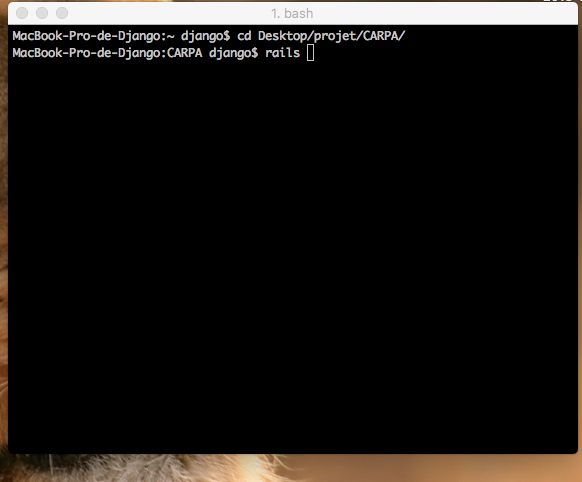
\includegraphics[width=0.7\linewidth]{terminal}
	\caption{Terminal}
	\label{fig:terminal}
\end{figure}


\begin{itemize}
	\item [\maltese] \textbf{Les modèles}  sont  des  classes  servant  à  modéliser  les données et à établir les relations entre elles. Cela permet d’établir le mapping entre les Objets et la base de données, grâce aux outils tels que \textbf{Active Record}. 
\end{itemize}
	Il est possible d'effectuer des requêtes de base sur les modèles.On trouve sur 
chaque modèles des méthodes save(), create(),find\_by\_name(),find() etc... Ces méthodes 
n'ont jamais été définies par le développeur, mais elles existent grâce au framework.\\
\indent Il  est  également  possible  de  contrôler  la  validation  des  formulaires  depuis le fichier qui définit le domaine.\\

\begin{itemize}
	\item [\maltese] \textbf{Les Contrôleurs}. Un contrôleur est une classe qui reçoit la requête de l'utilisateur et qui, en fonction de l'action demandée, va effectuer le traitement. 
\end{itemize}
\indent Pour gérer quelle est  l’action et quel contrôleur est appelé, Rails se base sur le formatage de l’URL: \textbf{: http://<…>/controller/action/}.\\
\begin{itemize}
	\item [\maltese] \textbf{Les Vues} sont représentées par un moteur de template \textbf{erb}, ou du \textbf{Haml}, on peut insérer du code Ruby.
	
	\indent On constate dans l'arborescence qu'il y'a une vue dédiée à chaque contrôleur et une vue dédiée à une action du contrôleur (Voir Annexe).
\end{itemize} 

\section{Le Langage Ruby}
Le langage Ruby a été conçu, au milieu des années 90, par Yukihiro Matsumoto, un
programmeur Japonais. Son objectif était d’avoir un langage qui soit « plaisant» à
utiliser: \\
\indent Ruby is \textbf{“made for developer happiness” !} (reference). \\C'est un Langage Orienté Objet. la figure.. présente un arbre généalogique de Ruby. Quant au tableau.. il représente les ancêtre de Ruby,avec les principales caractéristiques héritées de ces ancêtres. \\ \\
\begin{table}[h]
	\begin{center}
\begin{tabular}{|c|c|c|}
	\hline 
	\textbf{Langage} & \textbf{Année} & \textbf{Caractéristiques} \\ 
	\hline 
	Lisp & 1958  & approche fonctionnelle métaprogrammation \\ 
	\hline 
\textbf{CLU}	& 1974 & itérateurs  \\ 
	\hline 
	\textbf{Smalltalk}& 1980 & langage objet pur, blocs de code GUI, sUnit \\ 
	\hline 
Eiffel	&1986  &Uniform Access Principle  \\ 
	\hline 
  \textbf{Perl}	& 1987 & expressions régulières et pattern
  matching \\ 
	\hline 
\textbf{ Ruby}	& 1993  &  \\ 
	\hline 
\end{tabular}
\end{center}
\caption{Les ancêtres de Ruby.}
	\end{table} \\
La syntaxe de Ruby est faite pour apporter plus de flexibilité au framework Ruby On Rails
\begin{figure}[h]
	\centering
	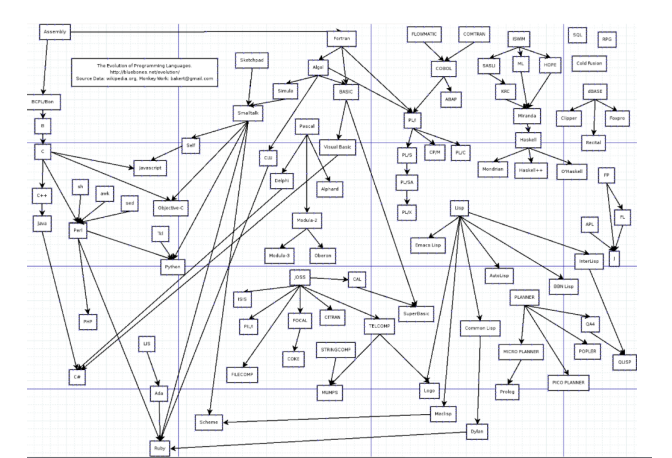
\includegraphics[width=0.7\linewidth]{arbregenea}
	\caption{Arbre généalogique de divers langages de programmation, incluant Ruby}
	\label{fig:arbregenea}
\end{figure}

\section{Architecture et Création d'un projet avec Ruby On Rails}

La création d'un projet ROR se fait en trois étapes:\\
		\begin{itemize}
	\item [\maltese] Création des classes de modèle;  
	\item [\maltese] Scaffolding ;
	\item [\maltese] Running.
\end{itemize}
\subsection{Création des classes de modèle}

Les «Migrations» sont des définitions du modèle. C’est la première étape dans la 
création d’un projet Rails. 

Nous avons utilisé dans ce projet la version \textbf{5.1.6}

La commande \textbf{ rails new nomProjet} permet de créer un projet nommé \textbf{nomProjet.}
  \textbf{Rails}  va  construire  un \textbf{nomProjet} avec  un  contenu  tel  que 
représenté par la figure.\\

Dès que le projet est créé, on se positionne à l’intérieur en invite de commande 
(cd nomProjet).  

La commande \textbf{rails generate modele Etudiant}  va créer un fichier \textbf{etudiant.rb} dans le dossier \textbf{app/models}


\begin{figure}[h]
	\centering
	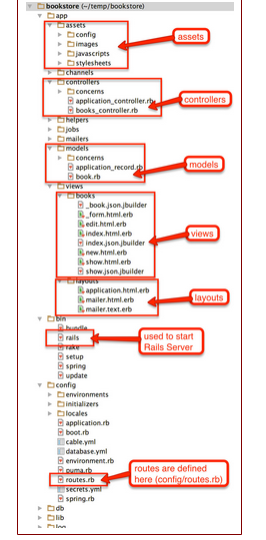
\includegraphics[width=0.5\linewidth]{arch}
	\caption{Contenu d’un dossier de projet Rails}
	\label{fig:arch}
\end{figure}

\newpage
\section{Scaffolding}
Le  scaffolding est une action de mise sur pied d’un échafaudage.  C’est là que 
repose la génération des futures fonctionnalités.

Il  se  gère  au  niveau  des  controllers et  permet  de  spécifier  les  actions  du 
contrôleur.

La  commande \textbf{rails} qui  permet  de  créer  un  contrôleur  pour  le  domaine 
Etudiant est : \textbf{rails generate controller Etududiants}. 

Un fichier  \textbf{EtudiantsController} sera créé dans le dossier  \textbf{app/controllers}.\\

Le \textbf{ scaffold}  prend  un  domaine  pour  lequel  le  contrôleur  définira les 
fonctionnalités CRUD. Ainsi, on pourra créer un  \textbf{Etudiant}, modifier ses champs et le supprimer ;  également,  l’affichage  de  la  liste  des  instances  d’\textbf{Etudiant} créées  sera disponible. 
\subsection{Running}
L’exécution d’un projet \textbf{rails} se fait par la commande \textbf{rails server}. On verra sur  la  console,  le  message  Server  Puma Booting 
\textbf{http://localhost:3000.}\\

\textbf{Rails}  nous  invite  ainsi  à  exécuter  l’application  sur  un  navigateur  à  l’adresse indiquée. Le navigateur nous présentera l’interface suivante :

\begin{figure}[h]
	\centering
	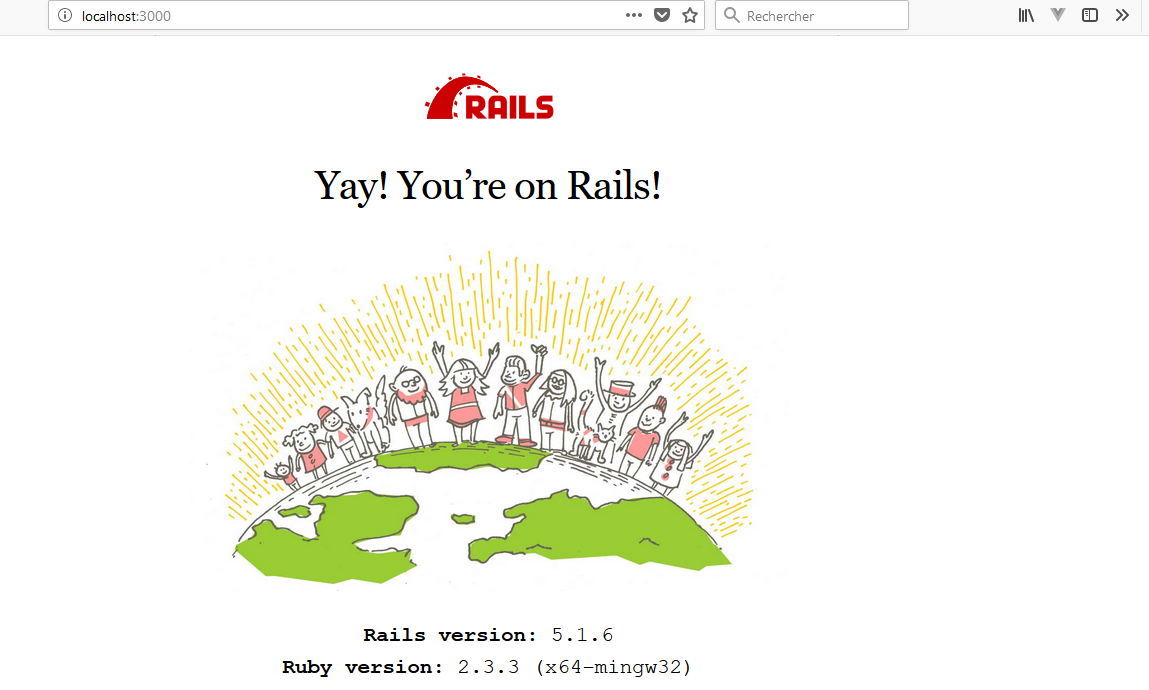
\includegraphics[width=0.7\linewidth]{rails}
	\caption{Première page d’un projet sur rails}
	\label{fig:rails}
\end{figure}

On  peut  constater  que  son  serveur  embarqué  utilise  par  défaut  le  port  3000. 
Mais, il peut être modifié si un autre serveur (tomcat par exemple) utilise déjà ce port. 
Dans ce cas, la commande d’exécution, pour le port 5050 par exemple, sera 
rails server.port=5050 . 

\section{ Avantages de Rails}
Les  avantages  que  l’on  peut  avoir  dans  l’utilisation  de  Grails  comme  RAD, 
peuvent être les suivants : 

\begin{itemize}
	
	\item [\textbullet] Web MVC : Facile à utiliser ;
	\item [\textbullet] ERB:  Langage de Template simple et complet ; 
	\item [\textbullet] Serveur embarqué ;
	\item [\textbullet] ActiveRecord: Modélisation et accès aux données ;
	\item [\textbullet] Base de données simulée (développement) ;
	\item [\textbullet] Internationalisation ;
	\item [\textbullet] Tests \& Tests unitaires ; 
	\item [\textbullet] Documentation très riche. 
\end{itemize}

\section{L'outil Git}

Il n’est pas toujours évident de parvenir rapidement au but que l’on se fixe dans 
la réalisation programmes. Pour ne pas rentre la tâche encore plus complexe, il peut 
être nécessaire d’utiliser des méthodes et outils permettant de ne pas s’éloigner du but. 
L'outils,  Git, que nous présentons dans cette partie nous permet de 
détecter les erreurs de régression et de gérer les versions, respectivement. 

\subsection{Git}
Toujours dans un souci d’efficacité et de rapidité,le programmeur ne doit pas 
se permettre une mauvaise gestion des versions. Une version est tout simplement l’état 
du  projet  à  un  moment  donné.  On  peut  toujours  avoir besoin,  dans  un  projet,  de 
retrouver un état antérieur.  Git est un outil qui permet de sauvegarder et de restaurer 
des états. 

Lorsque  \textbf{Git} est bien installé, pour commencer à suivre un projet existant dans 
 \textbf{Git}, il suffit de se positionner dans le répertoire du projet et exécuter la commande \textbf{git init}. Cela y va créer un sous-dossier nommé \textbf{.git}. 
La commande \textbf{ git add} fichier  permet d’indexer les fichiers du projet qui seront  suivis en version. 

Pour cloner un projet existant, on fait \textbf{git clone urlProjet. }
La  commande  \textbf{git  commit}  permet  de  valider  les  modifications  effectuées  sur  les fichiers indexés. 

Le  cycle  de  vie  des  états  d’un  fichier \textbf{Git} peut  être  illustré  par  la  figure  ci-dessous : 
\begin{figure}[h]
	\centering
	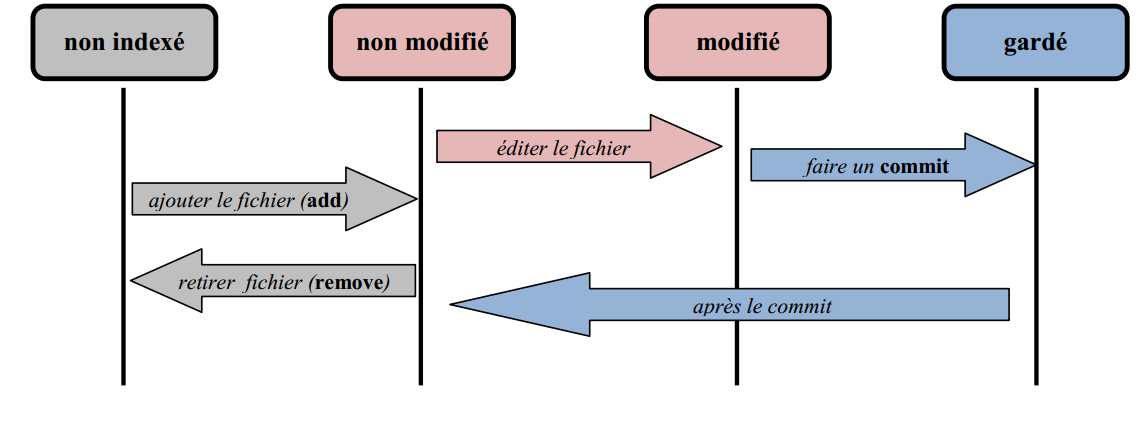
\includegraphics[width=0.7\linewidth]{git}
	\caption{Cycle de vie des états d’un fichier dans Git.}
	\label{fig:git}
\end{figure}

\section{ Le pattern MVC}
\subsection{Définition}
Un pattern est « une solution à un problème dans un contexte bien défini ». 
Ses quatre éléments d’un pattern sont : 
\begin{itemize}
	\item [\checkmark] son nom ; 
	\item [\checkmark] son but ; 
	\item [\checkmark] comment il résout le problème ; 
	\item [\checkmark] les contraintes à considérer dans la solution. \\
\end{itemize}
  
Les patterns nous permettent de réutiliser les solutions qui ont marché pour les 
autres ;  « pourquoi  réinventer  la  roue ? ».  Ils  nous  permettent  également  d’avoir  un vocabulaire commun. 
\subsection{Présentation du MVC}
MVC (Modèle – Vue  – Contrôleur) est un  design de  conception  d’interface 
utilisateur  permettant  de  découpler  le  modèle  (logique  métier  et  accès  aux  données) des vues (interfaces utilisateur). \\

Des modifications de l’un n’auront ainsi, idéalement, aucune conséquence sur l’autre ce qui facilitera grandement la maintenance. 

\subsection{Principe du MVC }
\textbf{Modèle: } gère les données et reprend la logique métier (le modèle lui même   peut   être  décomposé  en  plusieurs  couches  mais  cette  décomposition 
n'intervient  pas  au  niveau  de  MVC).  Le  modèle  ne  prend  en  compte  aucun 
élément de présentation ! \\

\textbf{Vue:}  elle  affiche  les  données,  provenant  exclusivement  du  modèle,  pour 
l'utilisateur et/ou reçoit ses actions. Aucun traitement, autre que la gestion de 
présentation, n'y est réalisé. \\

\textbf{Contrôleur:} son rôle est de traiter les événements en provenance de l’interface 
utilisateur  et  les  transmet  au  modèle  pour  le  faire évoluer  ou  à  la  vue  pour 
modifier son aspect visuel (pas de modification des données affichées mais des 
modifications de présentation). \\
Le contrôleur « connaît » la (les) vue(s) qu’il contrôle ainsi que le modèle. \\

Il  pourra  appeler  des  méthodes  du  modèle  pour  réagir  à  des  événements,  il 
pourra faire modifier à la vue son aspect visuel. Il pourra aussi instancier de nouvelles 
vues. Pour faire cela, le contrôleur sera à l'écoute d'événements survenant sur les vues. \\

La  vue  observera  le  modèle  qui  l'avertira  du  fait  qu'une  modification  est 
survenue. Dans ce cas, la vue interrogera le modèle pour obtenir son nouvel « état ». 
\begin{figure}[h]
	\centering
	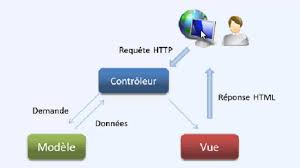
\includegraphics[width=0.8\linewidth]{mvc}
	\caption{Schématisation du MVC}
	\label{fig:mvc}
\end{figure}

\section{Constructeur d'un projet UML}
UML se définit comme un langage de modélisation graphique et textuel destiné 
à comprendre et décrire des besoins, spécifier et documenter des systèmes, esquisser 
des  architectures  logicielles,  concevoir  des  solutions  et  communiquer  des  points  de vue.\\

UML unifie à la fois les notations et les concepts orientés objet. Il ne s’agit pas 
d’une simple notation graphique, car les concepts transmis par un diagramme ont une 
sémantique précise et sont porteurs de sens au même titre que les mots d’un langage. \\

UML unifie également les notations nécessaires aux  différentes activités d’un 
processus  de  développement  et  offre,  par  ce  biais,  le  moyen  d’établir  le  suivi  des décisions prises, depuis l’expression de besoin jusqu’au codage. \\

Le  fil  tendu  entre  les  différentes  étapes  de  construction  permet  alors  de 
remonter du code aux besoins et d’en comprendre les tenants et les aboutissants. En 
d’autres termes, on peut retrouver la nécessité d’un bloc de code en se référant à son 
origine dans le modèle des besoins. \\

UML  2  s’articule  autour  de  treize  types  de  diagrammes,  chacun  d’eux  étant 
dédié à la représentation des concepts particuliers d’un système logiciel. Ces types de 
diagrammes sont répartis en deux grands groupes : 

\begin{itemize}
	\item [\maltese] diagrammes structurels: \\
\end{itemize}

\begin{itemize}
	\item [\textbullet] Diagramme  de  classes  –  Il  montre  les  briques  de  base  statiques  : classes,  associations,  interfaces,  attributs,  opérations,généralisations, etc. \\
	
	\item [\textbullet] Diagramme d’objets - Il montre les instances des éléments structurels et leurs liens à l’exécution.\\
	
	\item [\textbullet] Diagramme de packages - Il montre l’organisation logique du modèle et les relations entre packages.\\
	 
	\item [\textbullet] Diagramme  de  structure  composite  –  Il  montre  l’organisation  interne d’un élément statique complexe.\\
	
	\item [\textbullet] Diagramme de composants – Il montre des structures  complexes, avec 
	leurs interfaces fournies et requises.\\
	 
	\item [\textbullet] Diagramme de déploiement – Il montre le déploiement physique des « 
	artefacts » sur les ressources matérielles. 
	
\end{itemize}

\begin{itemize}
	
	\item [\maltese] Sept diagrammes comportementaux: \\
\end{itemize}

\begin{itemize}
	\item [\textbullet] Diagramme  de  cas  d’utilisation  -  Il  montre  les  interactions 
	fonctionnelles entre les acteurs et le système à l’étude. opérations,généralisations, etc. \\
	\item [\textbullet] Diagramme  de  vue  d’ensemble  des  interactions  -  Il  fusionne  les diagrammes  d’activité  et  de  séquence  pour  combiner  des  fragments 
	d’interaction avec des décisions et des flots.\\
	\item [\textbullet] Diagramme de séquence - Il montre la séquence verticale des messages passés entre objets au sein d’une interaction. 
	\item [\textbullet] Diagramme  de  communication  -  Il  montre  la  communication  entre objets dans le plan au sein d’une interaction\\
	\item [\textbullet] Diagramme  de  temps  –  Il  fusionne  les  diagrammes  d’états  et  de séquence  pour  montrer  l’évolution  de  l’état  d’un  objet  au  cours  du temps.\\ 
	\item [\textbullet] Diagramme  d’activité  -  Il  montre  l’enchaînement  des actions  et décisions au sein d’une activité.
	\item [\textbullet] Diagramme  d’états  –  Il  montre  les  différents  états  et  transitions possibles des objets d’une classe. 
\end{itemize}

\section{ Le Développement Agile }
\subsection{Les principes du Manifeste Agile }
La notion de méthode agile est née à travers un manifeste signé en 2001 par 17 
personnalités du développement logiciel. \\
Ce manifeste prône quatre valeurs fondamentales :
\begin{itemize}
	\item [\textbullet] «  Personnes  et  interactions  plutôt  que  processus  et  outils  »  :  dans  l’optique 
	agile, l’équipe est bien plus importante que les moyens matériels ou les procédures. Il 
	est  préférable  d’avoir  une  équipe  soudée  et  qui  communique,  composée  de 
	développeurs  moyens,  plutôt  qu’une  équipe  composée  d’individualistes,  même 
	brillants. La communication est une notion fondamentale. \\
\end{itemize}

\begin{itemize}
	\item [\textbullet] « Logiciel fonctionnel plutôt que documentation complète » : il est vital que 
	l’application  fonctionne.  Le  reste,  et  notamment  la documentation  technique,  est 
	secondaire, même si une documentation succincte et précise est utile comme moyen de 
	communication. La documentation représente une charge de travail importante et peut 
	être  néfaste  si  elle  n’est  pas  à  jour.  Il  est  préférable  de  commenter  abondamment  le 
	code  lui-même,  et  surtout  de  transférer  les  compétences  au  sein  de  l’équipe  (on  en 
	revient à l’importance de la communication). \\
\end{itemize}

\begin{itemize}
	\item  [\textbullet] « Collaboration avec le client plutôt  que négociation de contrat  » : le client 
	doit  être  impliqué  dans  le  développement.  On  ne  peut  se  contenter  de  négocier  un 
	contrat  au  début  du  projet,  puis  de  négliger  les  demandes  du  client.  Le  client  doit 
	collaborer avec l’équipe et fournir un feedback continu sur l’adaptation du logiciel à 
	ses attentes.\\
\end{itemize}

\begin{itemize}
	\item [\textbullet] « Réagir au changement plutôt que suivre un plan » : la planification initiale et 
	la  structure  du  logiciel  doivent  être  flexibles  afin  de  permettre  l’évolution  de  la 
	demande  du  client  tout  au  long  du  projet.  Les  premiers  releases  du  logiciel  vont 
	souvent provoquer des demandes d’évolution.
\end{itemize}

\subsection{La modélisation agile (AM) }
La « modélisation agile » prônée par Scott Ambler s’appuie sur des principes 
simples et de bon sens, parmi lesquels : 
\\
\begin{itemize}
	\item [\maltese]  Vous  devriez  avoir  une  grande  palette  de  techniques  à  votre  disposition  et 
	connaître  les  forces  et  les  faiblesses  de  chacune  de  manière  à  pouvoir  appliquer  la 
	meilleure au problème courant. \\
\end{itemize}

\begin{itemize}
	\item [\maltese] N’hésitez pas à changer de diagramme quand vous sentez que vous n’avancez 
	plus avec le modèle en cours. Le changement de perspective va vous permettre de voir 
	le  problème  sous  un  autre  angle  et  de  mieux  comprendre  ce  qui  bloquait 
	précédemment.\\ 
\end{itemize}
\begin{itemize}
	\item [\maltese] Vous trouverez souvent que vous êtes plus productif si vous créez plusieurs 
	modèles simultanément plutôt qu’en vous focalisant sur un seul type de diagramme. 
\end{itemize}

\section*{Conclusion}
Dans  ce  chapitre  de  généralités,  il  a  été  question  de  présenter  certains  outils 
utilisés dans le cadre de notre travail. Nous avons à cet effet présenté la technique du 
RAD, les outils Rails et Git, l’architecture MVC, le langage UML et la méthode 
de  développement  Agile.  Notons  également  que  tout  le  long  du  projet,  nous avons 
adopté une attitude « Agile », telle que décrite ci-dessus. 

\chapter{ANALYSE ET CONCEPTION}
 
\section*{Introduction}
Pour mettre sur pied un logiciel au sein d'une entreprise on passe par la réalisation d'un document appelé cahier de charges.\\

	\textrm{L'IEEE 1233 (ref ici) définit un cahier de charge comme étant l'expression d'un besoin à satisfaire. 
	Le cahier de charge n'indique pas la manière de réaliser le besoin, ni un produit à fournir,
	il est en amont de la conception. C'est donc le seul document qui décrit les besoins d'un utilisateur en termes de fonctions
	à assurer et d'objectifs atteindre.
}\\

Dans ce chapitre nous allons en  première phase  spécifier les besoins fonctionnels pour la mise en place d'une application du suivi de projet,du courrier et d'archivage numérique.
Cette phase  décrit  les  exigences  auxquelles  la  solution  à  mettre  en  place  devra 
répondre, en termes de fonctionnalités, de caractéristiques fonctionnelles attendues  et 
de la faisabilité du logiciel.
La  deuxième  phase  constituera  essentiellement  la  conception  de  notre  application.  Il  s’agira  de  l’établissement  du  diagramme  des  cas  d’utilisation,  des 
diagrammes de séquences et des diagrammes de classes pour mieux comprendre son fonctionnement, afin de maîtriser sa complexité et d'assurer sa cohérence.  \\

\section{Cahier de Charges}
\subsection{Fonctionnalités attendues de l'application}
Dans un début, il est important de recenser les propriétés fonctionnelles de de notre application. A la fin de ce projet notre application devrait être capable de:\\
\begin{itemize}
	\item 
\end{itemize}
\subsection{Besoins de l’application}
La spécification des besoins décrit sans ambiguïté l'application sécurisée à 
développer. L’énoncé d’un besoin exprime un comportement ou une propriété que 
le système doit respecter. Chaque énoncé traduit la présence d’un comportement très 
spécifique.

\begin{enumerate}
	\item  Un identifiant unique ;
	\item La catégorie du besoin qui décrit si celui-ci est fonctionnel ou non fonctionnel;
	\item La description ; 
	\item Une liste de termes le référant ;
	\item La justification de la présence et de l’utilité du besoin ;
	\item La priorité du besoin par l’une des appréciations suivantes: haute, moyenne, faible ;
	\item La vérification qui décrit un moyen avec lequel le client peut se rassurer  tel qu'implémenté, le besoin est remplie.
\end{enumerate} 
\subsection{Besoins fonctionnels}
Les besoins fonctionnels expriment des actions que doit effectuer l'application en 
réponse à une demande (sorties qui sont produites pour un ensemble donné d’entrées) . 
Pour mieux recenser ces besoins nous avons opté pour un découpage en module.\\

\begin{itemize}
	\item [\maltese] \textbf{Le module de gestion des utilisateurs}
\end{itemize}

\textrm{ Dans ce module nous pouvons énumérer les besoins suivants :}\\

\begin{itemize}
	\item [\textbullet] \textbf{Créer un utilisateur}\\
\end{itemize}

\begin{table}[h]
	\begin{center}
		\begin{tabular}{|c|c|}
			\hline 
			\textbf{Identifiant}&\textbf{F1 } \\ 
			\hline 
			\textbf{Catégorie } &fonctionnel  \\ 
			\hline 
			\textbf{Description}	& Le système permettra l’ajout des données des utilisateurs qui seront
			les futurs utilisateurs du système.   \\ 
			\hline 
			\textbf{Termes} & Administration, données, utilisateur \\ 
			\hline 
			\textbf{Justification} & Plusieurs  responsables du CARPA  utiliseront  l'application pour cela,  
			nous devons les  identifier  afin de leur créer des comptes 
			pour une bonne traçabilité \\ 
			\hline 
			\textbf{Priorité} 	& Haute \\ 
			\hline 
			\textbf{Vérification}	& Après enregistrement d’un utilisateur, on vérifie dans la liste  des 
			utilisateur si ce dernière existe \\ 
			\hline 
		\end{tabular} 
	\end{center}
\caption{Enregistrement d'un Utilisateur} 
\end{table}

\begin{itemize}
	\item [\textbullet]\textbf{ Modifier un utilisateur}\\
\end{itemize}

\begin{table}[h]
	\begin{center}
		\begin{tabular}{|c|c|}
			\hline 
			\textbf{Identifiant} & \textbf{ F2} \\ 
			\hline 
		\textbf{Catégorie }	& fonctionnel  \\ 
			\hline 
		\textbf{Description }	& Le système permettra de modifier les données d’un utilisateur. \\ 
			\hline 
			\textbf{Termes }& Administration, données, utilisateur, modification \\ 
			\hline 
		\textbf{Justification }	&  L’administrateur peut mal saisir les données\\ 
			\hline 
			\textbf{Priorité }& Moyenne \\ 
			\hline 
			\textbf{Vérification }& Après  la modification  d’un utilisateur, on vérifie dans la liste des utilisateurs si la modification est effective. \\ 
			\hline 
		\end{tabular} 
	\end{center}
\caption{Modifier un utilisateur}
\end{table}
\newpage
\begin{itemize}
	\item [\textbullet] \textbf{Supprimer un utilisateur}\\
\end{itemize}
 
 \begin{table}[h]
 	\begin{center}
 		\begin{tabular}{|c|c|}
 			\hline 
 			\textbf{Identifiant }& \textbf{F3} \\ 
 			\hline 
 			\textbf{Catégorie }& fonctionnel \\ 
 			\hline 
 			\textbf{Description }& Supprimer un utilisateur \\ 
 			\hline 
 		\textbf{Termes }	& Administration, données, utilisateur, suppression \\ 
 			\hline 
 			\textbf{Justification }& Le CARPA peut décider de rompre le contrat de un des responsable ou ce dernier peut être mis à la retraite  \\ 
 			\hline 
 		\textbf{Priorité }	& Moyenne \\ 
 			\hline 
 			\textbf{Vérification }& Après la suppression  d’un utilisateur, on vérifie  si l'utilisateur  n’est plus dans la liste \\ 
 			\hline 
 		\end{tabular} 
 	
 	\end{center}
 \caption{Suppression d'un Utilisateur}
 \end{table}

\begin{itemize}
	\item [\textbullet] \textbf{Créer un compte d’utilisateur}\\
\end{itemize}

\begin{table}[h]
	\begin{center}
		\begin{tabular}{|c|c|}
			\hline 
			\textbf{Identifiant}	& \textbf{F4} \\ 
			\hline 
			\textbf{Catégorie }	&  fonctionnel\\ 
			\hline 
			\textbf{Description }	& Le système permettra l’ajout des comptes d’utilisateurs. \\ 
			\hline 
			\textbf{Termes }	&  Administration, donnée, compte\\ 
			\hline 
			\textbf{Justification }	& Plusieurs  utilisateurs sont dans le système et chacun doit avoir 
			un compte pour se connecter à l’application.   \\ 
			\hline 
			\textbf{Priorité }&Haute  \\ 
			\hline 
			\textbf{Vérification }	& Après enregistrement d’un compte, on vérifie dans la liste des 
			comptes si ce dernier existe. \\ 
			\hline 
		\end{tabular} 
	\end{center}
	\caption{Enregistrer un compte utilisateur}
\end{table}

\begin{itemize}
	\item [\textbullet] \textbf{Modifier un compte }\\
\end{itemize}

\begin{table}[h]
	\begin{center}
		\begin{tabular}{|c|c|}
			\hline 
			\textbf{Identifiant}	& \textbf{F5} \\ 
			\hline 
			\textbf{Catégorie }	&  fonctionnel\\ 
			\hline 
			\textbf{Description }	& Le système permettra de modifier les données d’un compte.\\ 
			\hline 
			\textbf{Termes }	&  Administration, donnée, compte, modification\\ 
			\hline 
			\textbf{Justification }	& L’administrateur peut mal saisir les données, ou alors le profil
			de l’utilisateur peut changer.    \\ 
			\hline 
			\textbf{Priorité }&Moyenne  \\ 
			\hline 
			\textbf{Vérification }	& Après la modification d’un compte, on vérifie dans la liste des 
			comptes si ce dernier existe. \\ 
			\hline 
		\end{tabular} 
	\end{center}
	\caption{Enregistrer un compte utilisateur}
\end{table}

\begin{itemize}
	\item [\textbullet] \textbf{Effectuer des recherches sur les utilisateurs }\\
\end{itemize}

\begin{table}[h]
	\begin{center}
		\begin{tabular}{|c|c|}
			\hline 
			\textbf{Identifiant}	& \textbf{F6} \\ 
			\hline 
			\textbf{Catégorie }	&  fonctionnel\\ 
			\hline 
			\textbf{Description }	&Le  système  permettra  de   faire  une   recherche  rapide  sur  les 
			utilisateurs.\\ 
			\hline 
			\textbf{Termes }	& Administration, données, utilisateur, modification, recherche.\\ 
			\hline 
			\textbf{Justification }	& L’administrateur  peut  avoir  besoin  des  informations  sur  une 
			personne.    \\ 
			\hline 
			\textbf{Priorité }&Moyenne  \\ 
			\hline 
			\textbf{Vérification }	& Si la personne existe dans le système alors elle sera affichée. \\ 
			\hline 
		\end{tabular} 
	\end{center}
	\caption{Rechercher un utilisateur}
\end{table}
\newpage
\begin{itemize}
	\item [\maltese] \textbf{Le module de gestion du courrier}
\end{itemize}



\begin{table}[h]
	\begin{center}
		\begin{tabular}{|c|c|}
			\hline 
			\textbf{Identifiant}	& \textbf{F7} \\ 
			\hline 
			\textbf{Catégorie }	&  fonctionnel\\ 
			\hline 
			\textbf{Description }	&Le  système  permettra  de   faire  une   recherche  rapide  sur  les courriers.\\ 
			\hline 
			\textbf{Termes }	& Administration, données,  courrier.\\ 
			\hline 
			\textbf{Justification }	& L’administrateur ou l'utilisateur  peut  avoir  besoin  des  informations sur un courrier.    \\ 
			\hline 
			\textbf{Priorité }&Haute  \\ 
			\hline 
			\textbf{Vérification }	& Si le courrier existe dans le système alors il sera affiché. \\ 
			\hline 
		\end{tabular} 
	\end{center}
	\caption{Enregistrer un courrier}
\end{table}


\begin{itemize}
	\item [\textbullet] \textbf{Modifier un courrier}
\end{itemize}

\begin{table}[h]
	\begin{center}
		\begin{tabular}{|c|c|}
			\hline 
			\textbf{Identifiant}	& \textbf{F8} \\ 
			\hline 
			\textbf{Catégorie }	&  fonctionnel\\ 
			\hline 
			\textbf{Description }	&Le  système  permettra  de   faire  une  modification sur  les courriers.\\ 
			\hline 
			\textbf{Termes }	& Administration, données,  courrier, modification.\\ 
			\hline 
			\textbf{Justification }	& L’administrateur ou l'utilisateur  peut  avoir  besoin  des  informations sur un courrier.    \\ 
			\hline 
			\textbf{Priorité }& Moyenne  \\ 
			\hline 
			\textbf{Vérification }	& Après la modification, on vérifie dans la liste des courriers si ce dernier est à jour. \\ 
			\hline 
		\end{tabular} 
	\end{center}
	\caption{Modifier un courrier}
\end{table}

\begin{itemize}
	\item [\textbullet]  \textbf{Supprimer un courrier}
\end{itemize}


\begin{table}[h]
	\begin{center}
		\begin{tabular}{|c|c|}
			\hline 
			\textbf{Identifiant}	& \textbf{F9} \\ 
			\hline 
			\textbf{Catégorie }	&  fonctionnel\\ 
			\hline 
			\textbf{Description }	&Le  système  permettra  de   faire  la suppression d'un courrier.\\ 
			\hline 
			\textbf{Termes }	& Administration, données,  courrier, suppression.\\ 
			\hline 
			\textbf{Justification }	& CARPA peut décider de ne plus avoir besoin des informations d'un courrier.    \\ 
			\hline 
			\textbf{Priorité }& Moyenne  \\ 
			\hline 
			\textbf{Vérification }	& Après la suppression , on vérifie dans la liste des courriers si ce dernier  a été supprimer. \\ 
			\hline 
		\end{tabular} 
	\end{center}
	\caption{Supprimer un courrier}
\end{table}

\newpage
\begin{itemize}
	\item [\maltese] \textbf{Le module suivi des projets}\\
\end{itemize}

\begin{itemize}
	\item [\textbullet]  \textbf{Enregistrer un projet}
\end{itemize}



\begin{table}[h]
	\begin{center}
		\begin{tabular}{|c|c|}
			\hline 
			\textbf{Identifiant}	& \textbf{F10} \\ 
			\hline 
			\textbf{Catégorie }	&  fonctionnel\\ 
			\hline 
			\textbf{Description }	&Le  système  permettra  de   faire  l'enregistrement d'un projet.\\ 
			\hline 
			\textbf{Termes }	& Administration, données,  projet.\\ 
			\hline 
			\textbf{Justification }	& L'administrateur a besoin des données qui permettrons de faire le suivi des projets   \\ 
			\hline 
			\textbf{Priorité }& Haute \\ 
			\hline 
			\textbf{Vérification }	& Après l'enregistrement , on se rassure que ce dernier se est bien dans la liste. \\ 
			\hline 
		\end{tabular} 
	\end{center}
	\caption{Enregistrer un projet}
\end{table}

\begin{itemize}
	\item [\textbullet]  \textbf{Modification d'un projet}
\end{itemize}

\begin{table}[h]
	\begin{center}
		\begin{tabular}{|c|c|}
			\hline 
			\textbf{Identifiant}	& \textbf{F11} \\ 
			\hline 
			\textbf{Catégorie }	&  fonctionnel\\ 
			\hline 
			\textbf{Description }	&Le  système  permettra  de   faire  la modification d'un projet.\\ 
			\hline 
			\textbf{Termes }	& Administration, données,  projet, modification.\\ 
			\hline 
			\textbf{Justification }	& L'administrateur ou l'utilisateur peut faire une erreur dans la saisie d'une d'un projet et souhaite faire une modification    \\ 
			\hline 
			\textbf{Priorité }& Moyenne\\ 
			\hline 
			\textbf{Vérification }	& Après la modification d'une phase du projet, on verifie s'il est dans la liste des phases du projet. \\ 
			\hline 
		\end{tabular} 
	\end{center}
	\caption{Modifier un projet}
\end{table}

\begin{itemize}
	\item [\textbullet] \textbf{Supprimer un projet}
\end{itemize}
\newpage



\begin{table}[h]
	\begin{center}
		\begin{tabular}{|c|c|}
			\hline 
			\textbf{Identifiant}	& \textbf{F12} \\ 
			\hline 
			\textbf{Catégorie }	&  fonctionnel\\ 
			\hline 
			\textbf{Description }	&Le  système  permettra  de   faire  la suppresion d'un projet.\\ 
			\hline 
			\textbf{Termes }	& Administration, données,  projet, suppresion.\\ 
			\hline 
			\textbf{Justification }	& CARPA peut décider de ne plus avoir besoin des informations d'un projet    \\ 
			\hline 
			\textbf{Priorité }& Moyenne\\ 
			\hline 
			\textbf{Vérification }	& Après la suppression, on vérifie dans la liste des projets  si ce dernier a disparu. \\ 
			\hline 
		\end{tabular} 
	\end{center}
	\caption{supprimer un projet}
\end{table}


\begin{itemize}
	\item [\maltese] \textbf{Le module gestion des phase du projet}\\
\end{itemize}

\begin{itemize}
	\item [\textbullet] \textbf{Enregistrer une phase du projet}\\ 
\end{itemize}

\begin{table}[h]
	\begin{center}
		\begin{tabular}{|c|c|}
			\hline 
			\textbf{Identifiant}	& \textbf{F13} \\ 
			\hline 
			\textbf{Catégorie }	&  fonctionnel\\ 
			\hline 
			\textbf{Description }	&Le  système  permettra  de   faire  l'enregistrement d'une phase du projet.\\ 
			\hline 
			\textbf{Termes }	& Administration, données,  phase projet.\\ 
			\hline 
			\textbf{Justification }	& L'administrateur ou l'utilisateur  a besoin des données concernant les phase du projet pour le suivi des projets.   \\ 
			\hline 
			\textbf{Priorité }& Haute\\ 
			\hline 
			\textbf{Vérification }	& Après l'enregistrement , on vérifie dans la liste des  phases du projet   ce dernier est bien enregistrée . \\ 
			\hline 
		\end{tabular} 
	\end{center}
	\caption{Enregistrer une phase du projet}
\end{table}


\begin{itemize}
	\item [\textbullet] \textbf{Modifier une phase du projet} \\ 
\end{itemize}


\begin{table}[h]
	\begin{center}
		\begin{tabular}{|c|c|}
			\hline 
			\textbf{Identifiant}	& \textbf{F14} \\ 
			\hline 
			\textbf{Catégorie }	&  fonctionnel\\ 
			\hline 
			\textbf{Description }	&Le  système  permettra  de   faire  la modification d'une phase du projet.\\ 
			\hline 
			\textbf{Termes }	& Administration, données,  phase du projet, modification.\\ 
			\hline 
			\textbf{Justification }	& L'administrateur ou l'utilisateur peut faire une erreur dans la saisie d'une phase du projet et souhaite une modification    \\ 
			\hline 
			\textbf{Priorité }& Moyenne\\ 
			\hline 
			\textbf{Vérification }	& Après la modification d'une phase du projet, on verifie s'il est dans la liste des phases du projet. \\ 
			\hline 
		\end{tabular} 
	\end{center}
	\caption{Modifier un projet}
\end{table}

\begin{itemize}
	\item [\textbullet] \textbf{Supprimer une phase du projet}
\end{itemize}

\newpage

	\begin{table}[h]
	\begin{center}
	\begin{tabular}{|c|c|}
		\hline 
		\textbf{Identifiant}	& \textbf{F15} \\ 
		\hline 
		\textbf{Catégorie }	&  fonctionnel\\ 
		\hline 
		\textbf{Description }	&Le  système  permettra  de   faire  la suppresion d'une phase du projet.\\ 
		\hline 
		\textbf{Termes }	& Administration, données,  phase du projet, suppresion.\\ 
		\hline 
		\textbf{Justification }	& CARPA peut décider de ne plus avoir besoin des informations d'une phase du projet    \\ 
		\hline 
		\textbf{Priorité }& Moyenne\\ 
		\hline 
		\textbf{Vérification }	& Après la suppression, on vérifie dans la liste des phase du projet  si ce dernier a disparu. \\ 
		\hline 
	\end{tabular} 
  \end{center}
  	\caption{supprimer une phase du projet}
\end{table}

\begin{itemize}
	\item [\maltese] \textbf{Le module archivage}\\
\end{itemize}

\begin{itemize}
	\item [\textbullet] \textbf{Enregistrer une Archive}\\
\end{itemize}

\begin{table}[h]
	\begin{center}
		\begin{tabular}{|c|c|}
			\hline 
			\textbf{Identifiant}	& \textbf{F16} \\ 
			\hline 
			\textbf{Catégorie }	&  fonctionnel\\ 
			\hline 
			\textbf{Description }	&Le  système  permettra  de   faire  l'enregistrement d'une archive.\\ 
			\hline 
			\textbf{Termes }	& Administration, données,  archive.\\ 
			\hline 
			\textbf{Justification }	& L'administrateur ou l'utilisateur  a besoin des données concernant les archives.   \\ 
			\hline 
			\textbf{Priorité }& Haute\\ 
			\hline 
			\textbf{Vérification }	& Après l'enregistrement , on vérifie dans la liste des  archives si  ce dernier est bien enregistrée . \\ 
			\hline 
		\end{tabular} 
	\end{center}
	\caption{Enregistrer une archive}
\end{table}


\begin{itemize}
	\item [\textbullet] \textbf{Modifier une phase du projet} \\ 
\end{itemize}


\begin{table}[h]
	\begin{center}
		\begin{tabular}{|c|c|}
			\hline 
			\textbf{Identifiant}	& \textbf{F17} \\ 
			\hline 
			\textbf{Catégorie }	&  fonctionnel\\ 
			\hline 
			\textbf{Description }	&Le  système  permettra  de   faire  la modification d'une archive.\\ 
			\hline 
			\textbf{Termes }	& Administration, données,  archive, modification.\\ 
			\hline 
			\textbf{Justification }	& L'administrateur ou l'utilisateur peut faire une erreur dans l'enregistrement d'une archive et souhaite une modification    \\ 
			\hline 
			\textbf{Priorité }& Moyenne\\ 
			\hline 
			\textbf{Vérification }	& Après la modification d'une archive, on verifie s'il est dans la liste des archive. \\ 
			\hline 
		\end{tabular} 
	\end{center}
	\caption{Modifier une archive}
\end{table}


\begin{itemize}
	\item [\textbullet] \textbf{Supprimer une archive} \\ 
\end{itemize}
\newpage

\begin{table}[h]
	\begin{center}
		\begin{tabular}{|c|c|}
			\hline 
			\textbf{Identifiant}	& \textbf{F15} \\ 
			\hline 
			\textbf{Catégorie }	&  fonctionnel\\ 
			\hline 
			\textbf{Description }	&Le  système  permettra  de   faire  la suppresion d'une archive\\ 
			\hline 
			\textbf{Termes }	& Administration, données,  archive, suppresion.\\ 
			\hline 
			\textbf{Justification }	& CARPA peut décider de ne plus avoir besoin des informations concernant une archive.   \\ 
			\hline 
			\textbf{Priorité }& Moyenne\\ 
			\hline 
			\textbf{Vérification }	& Après la suppression, on vérifie dans la liste des archive  si ce dernier a disparu. \\ 
			\hline 
		\end{tabular} 
	\end{center}
	\caption{supprimer une archive}
\end{table}


\begin{itemize}
	\item [\maltese] \textbf{Le module administration des données}\\
\end{itemize}

\begin{itemize}
	\item [\textbullet] \textbf{Importer les données sous format excel, pdf, doc etc} \\ 
\end{itemize}

\begin{table}[h]
	\begin{center}
		\begin{tabular}{|c|c|}
			\hline 
			\textbf{Identifiant}	& \textbf{F15} \\ 
			\hline 
			\textbf{Catégorie }	&  fonctionnel\\ 
			\hline 
			\textbf{Description }	&Le  système  permettra  aux utilisateurs d'importer les données sous format excel, pdf, doc etc.\\ 
			\hline 
			\textbf{Termes }	& Administration, données,  importé.\\ 
			\hline 
			\textbf{Justification }	& Ceci facilite l'administration des données et la production des rapports.   \\ 
			\hline 
			\textbf{Priorité }& Moyenne\\ 
			\hline 
			\textbf{Vérification }	& Après importation des données, ces dernières apparaissent dans la liste. \\ 
			\hline 
		\end{tabular} 
	\end{center}
	\caption{Importer les données}
\end{table}


\begin{itemize}
	\item [\textbullet] \textbf{Exporter les données sous format excel, pdf, json, xml} \\ 
\end{itemize}

\begin{table}[h]
	\begin{center}
		\begin{tabular}{|c|c|}
			\hline 
			\textbf{Identifiant}	& \textbf{F15} \\ 
			\hline 
			\textbf{Catégorie }	&  fonctionnel\\ 
			\hline 
			\textbf{Description }	&Le  système  permettra  aux utilisateurs d'exporter les données sous format excel, pdf, json, xml .\\ 
			\hline 
			\textbf{Termes }	& Administration, données,  exporté.\\ 
			\hline 
			\textbf{Justification }	& Ceci facilite  la production des rapports.   \\ 
			\hline 
			\textbf{Priorité }& Moyenne\\ 
			\hline 
			\textbf{Vérification }	& Après l'exportation un document est produit en fonction du format choisis. \\ 
			\hline 
		\end{tabular} 
	\end{center}
	\caption{Exporter les données}
\end{table}

\subsection{Besoins non fonctionnels}

Les besoins non spécifiques sont des besoins qui font références aux aspects généraux de l'interface utilisateur. ce sont des besoins en matière de performance, de type de materiel ou le type de conception.\\

\begin{itemize}
	\item [\checkmark] \textbf{Ergonomie et convivialité}\\
\end{itemize}

\textrm{L'application devra disposer d'une interface conviviale, facile et agréable à utiiser et à comprendre, permettant ainsi une appropriation rapide et intuitive par ses utilisateurs. Le portail doit être simple et transparent, laissant les utilisateurs prendre le contrôle de l'application.}\\

\begin{itemize}
	\item [\checkmark] \textbf{Sécurité et fiabilité}\\
\end{itemize}

\textrm{L'application devra envoyer des notifications pour toutes tentatives d'usurpation des droits de privilèges ou lorsqu'un champs est mal rempli. L'application devra restreintre l'utilisation de ses fonctionnalités sur le principe de responsabilité des utilisateurs et des moindres privilèges. Le droit d'accès aux ressources doit se fonder sur le principe de moindres privilèges  et de la responsabilité des utilisateurs.\\ }
\begin{itemize}
	\item [\checkmark] \textbf{Documentation}\\
\end{itemize}

\textrm{L'application devra être documentée:\\
	\begin{itemize}
		\item [\maltese] Au niveau du code proprement dit (commentaire des lignes de code), pour permettre en cas de besoin de comprendre, modifier ou changer le code; ceci nous permet d'assurer la maintenance qui est l'une des bonnes qualités d'un logiciel.\\
		\item [\maltese] Au niveau de l'interface, considerée comme aide dans notre cas, elle permet à tout utilisateur de mieux s'accommoder aux portail afin d'assurer l'utilisabilité.\\
		Les documents qui accompagneront la livraison de l'application sont:\\
		 \item [\textbullet] Document de conception;
		 \item [\textbullet] Document  de modelisation;
		 \item [\textbullet] Guide de l'utilisation.
	\end{itemize}
}
\begin{itemize}
	\item [\checkmark] \textbf{Evolution, maintenance et réutilisation}\\
\end{itemize}

\textrm{Pour faciliter l’évolutivition, la réutilisation et la maintenance, l’application devra
être développée suivant une architecture choisie sur la base des technologies utilisées
pour son développement ; mais aussi, la séparation en module devra être prise en compte
pour mieux cerner les fonctionnalités qui y sont implémentées. Et enfin les conventions
de codage telles que l’utilisation des noms significatifs, majuscules pour les constantes
etc. devront être respectées.}

\subsection{Etude de faisabilité}
   \subsubsection{3.1.5.1 Justification du projet}
   \textrm{La mise en place de cette plateforme permettra à l'entreprise de profiter au maximun des avantages suivants:\\}
   
   \begin{itemize}
   	\item [\checkmark] \textbf{Gagner en temps et limiter les coûts et dépenses:} Tous les membres de
l’entreprise signaleront à temps les différents problèmes rencontrés et ceux-ci
seront pris en charge et résolus dans les brefs délais. \\ 
   \end{itemize}

\begin{itemize}
	\item [\checkmark] \textbf{Augmenter la productivité :} il est clair que la résolution des problèmes à temps
et dans les brefs délais augmente la productivité de l’entreprise.\\
\end{itemize}
	\subsubsection{3.1.5.2 Analyse des coûts et bénefices}
	\textrm{Les bénéfices de l’utilisation d’une telle application ont déjà été énumérés dans le
paragraphe précédent. Cependant, en termes de coûts :}
	\subsubsection{3.1.5.3 Planning prévisionnel}

\chapter{IMPLÉMENTATION}
\section{Introduction}
 Dans ce chapitre nous entamons la partie pratique, ou nous allons présenter l’environnement et les outils de développement utilisé, l’architecture de l’application et quelques interfaces de celui-ci. Vue la complexité de notre système après analyse, conception et modélisation il ne sera évident pour nous de l'implémenter comme cela a été prévu dans le cahier de charge tout en respectant les délais prescrit.En se basant sur l'étude de l'existant faite au \textbf{chapitre 2} dans les généralités, nous avons opté pour l'utilisation d'une solution open source qui couvre le maximum de fonctionnalités exigées, et la modification pour satisfaire aux besoins de l'entreprise.
\section{Langages de programmation et Environnement de développement}
	\subsection{Langages de programmation et Framework}
 \begin{enumerate}
 	\item \textbf{Ruby}\\
 	Le langage Ruby a été conçu, au milieu des années 90, par Yukihiro Matsumoto, un
 	programmeur Japonais. Son objectif était d’avoir un langage qui soit « plaisant» à
 	utiliser, (référence ici) c'est un langage open source dynamique et orienté objet avec une syntaxe flexible. La version utilisée est la \textbf{2.5.1}.\\
 	
 \indent	Le langage Ruby compte diverses manières d’utilisation(référence ici):
 	\begin{itemize}
 		\item Pour une interface web : c’est l’utilisation la plus courante ;
 		\item En ligne de commandes (CLI "Command Line Interface") ;
 		\item Pour produire une interface desktop (GUI "Graphical User Interface ").\\
 	\end{itemize}
   	\item \textbf{JavaScript}\\
   	JavaScript est un langage de script orienté objet principalement utilisé dans les pages HTML.
   	A l’opposé des langages serveurs (qui s’exécutent sur le site), Javascript est exécuté sur l’ordinateur de l’internaute par le navigateur lui-même. Ainsi, ce langage permet une interaction
   	avec l’utilisateur en fonction de ses actions (lors du passage de la souris au dessus d’un élément,
   	du redimensionnement de la page, etc). La version standardisée de Javascript est l’ECMAScript.(référence ici)\\
   	\item \textbf{HTML/XHTML}\\
   	 Le HTML et sa variante plus stricte XHTML sont des langages de balisage 
   	des   pages  Web.  Il  n’y  a  pas  si  longtemps,  le  HTML  servait  à  définir  aussi  bien  la 
   	structure des pages que leur présentation visuelle. Aujourd'hui, ces deux aspects doivent 
   	être bien distincts et le X/HTML est destiné uniquement à représenter la structure d’une 
   	page : titres, sous-titres, paragraphes, images, formulaires de saisie, liens hypertextes, 
   	etc.\\
   	
   	\item \textbf{CSS}\\
   	CSS (Cascading Style Sheets, ou feuilles de styles en cascade) permet de 
   	modifier la présentation des éléments X/HTML : couleur, taille, police de caractères, 
   	mais aussi  position sur la page, largeur, hauteur, empilement, bref tout ce qui 
   	touche à la mise en page d’un document X/HTML.\\
   	
   	\item \textbf{Bootstrap}\\
   	Bootstrap est un framework CSS, mais pas seulement, puisqu’il embarque également des
   	composants HTML et JavaScript. Il comporte un système de grille simple et efficace pour mettre
   	en ordre l’aspect visuel d’une page web. Il apporte du style pour les boutons, les formulaires,
   	la navigation...etc.Il permet ainsi de concevoir un site web rapidement et avec peu de lignes de code ajoutées. Le framework le plus proche de Bootstrap est sans doute Foundation qui est
   	présenté comme « The most advanced responsive front-end framework in the world » (référence ici) \\
   	
   	\item \textbf{Ruby On Rails}\\
   	{Ruby On Rails est un framework libre distribué sous licence MIT destiné au prototypage et au  développement d'application Web diverses et variées, il est multiplateforme . 
   	ROR (Ruby On Rails) est orienté RAD (Rapid Application Development)(reference ici)},
   	il reprend de nombreux principes communs aux méthodes "Agiles" et est 
   	basé sur l'architecture MVC et ceci se voit dès l'arborescence d'un projet ROR .\\
   	
   	\item \textbf{JQUERY}\\
   	jQuery est un framework JavaScript libre et Open Source, implanté côté client, qui
   	porte sur l’interaction entre le DOM(Document Object Model), JavaScript, AJAX et
   	le Html. Cette librairie JavaScript a pour but de simplifier les commandes communes du
   	JavaScript. La devise de jQuery est en effet, "Écrire moins pour faire plus" (write less do more).\\
   	
   	jQuery, du moins à l’origine, est l’œuvre d’un seul homme : John Resig. Ce jeune surdoué
   	de JavaScript développa la première version de jQuery en janvier 2006.\\
   	
   	Les spécificités de jQuery sont nombreuses mais l’essentielle est assurément la souplesse qu’il apporte pour accéder à tous les éléments du document Html grâce à la multitude de sélecteurs mis en place. Cette caractéristique fut d’ailleurs retenue pour donner un nom à ce framework :
   	j pour JavaScript et Query pour chercher ou accéder aux éléments.(reference ici)\\
   	
   	\item \textbf{XML}\\
   	XML  (eXtensible   Markup   Language)   est   un   langage   de   balisage,   qui   se 
   	distingue de HTML par le fait qu'il permet de spécifier la structure du contenu d'un 
   	document plutôt que la façon de le présenter.\\
   	
   	\item \textbf{SQL}
   	SQL  (Structured Query Language) est un langage d'interrogation de base de données 
   	très populaire. Il constitue aujourd'hui une norme implémentée par de nombreux SGBD 
   	(Systèmes de Gestion de Bases de Données).
 \end{enumerate}

\subsection{Outils de développement}

\begin{enumerate}
	\item \textbf{SQLITE}\\
	Sqlite est le système de gestion de base de données (SGBD) que nous avons utilisé 
	pour gérer notre base de données car il respecte le modèle d'architecture 3-tiers. 
	Il permet de créer facilement nos tables, il est sécurisé, rapide et léger,	
	qui fonctionne sur de nombreux  systèmes  d’exploitation  (dont  Linux,  Mac  OS,  Windows,  Solaris, FreeBSD…)  et  qui  est  accessible  en  écriture  par  de  nombreux  langages  de programmation, incluant notamment Ruby, C, C++ ,PHP, Java, .NET, Python .\\
	
	\item \textbf{ RubyMine}\\
	 RubyMine est un environnement de développement intégré (IDE), 
	qui est cross-plateform (utilisable sur n'importe quel système), 
	il comprend toutes les caractéristiques d'un IDE moderne (éditeur couleur, projet multiplateforme et de page web) intègre le système de contrôle de version
	et bien d'autre outils  à son sein, il est payant mais néanmoins donne une version d'essai de 30 jours et une licence pour étudiant.\\
	
	\item \textbf{ImageMagick}\\
	ImageMagick est un logiciel en ligne de commande très puissant de manipulation d'image dans pratiquement tous les formats existant.
	Sa licence est compatible avec la licence GPL (general public licence).\\
	
	\item \textbf{StarUml}
StarUml est un	logiciel de modélisation UML, qui nous a permis de modéliser nos différents diagrammes
\end{enumerate}

\section{Présentation du projet}
L’arborescence  du  projet  représente  ici  l’empaquetage  et  l’organisation  des 
différents  fichiers  du  projet.  Le  projet  Java  que  nous  avons  créé  sur RubyMine  est constitué  en module,  en  fonction  de  leurs  utilités.  Les  captures  ci-dessous présentent cette arborescence, d’abord dans un explorateur Windows, et ensuite dans l’IDE RubyMine.
\begin{figure}[h]
	\centering
	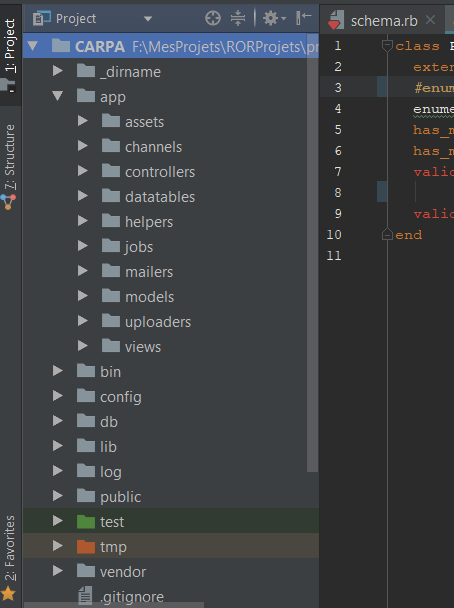
\includegraphics[width=0.4\linewidth]{aborescence}
	\caption{Arborescence du projet dans l'IDE RubyMine}
	\label{fig:aborescence}
\end{figure}

\begin{figure}[h]
	\centering
	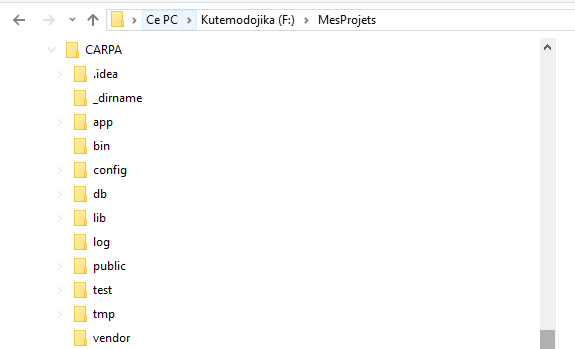
\includegraphics[width=0.5\linewidth]{explorateur}
	\caption{Arborescence du projet dans l'explorateur windows}
	\label{fig:explorateur}
\end{figure}

\section{Modèle Architectural}
\subsection{Synoptique de fonctionnement d'une application web}

La figure ci-dessous  présente le principe de fonctionnement de notre  application 
web. Dans cette architecture,  nous avons  d’un côté, un ordinateur  ayant notre application web et de l’autre, un serveur qui communique avec notre ordinateur à travers des web services.
\begin{figure}[h]
	\centering
	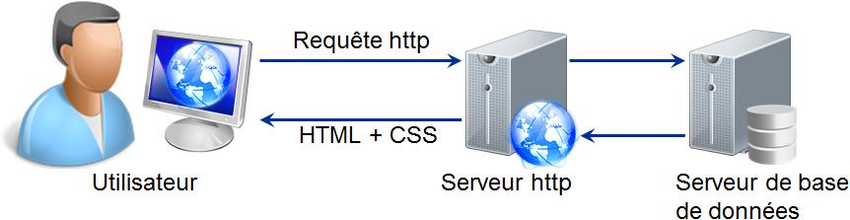
\includegraphics[width=0.7\linewidth]{web}
		\caption{Synoptique de l'application web}
	\label{fig:web}
\end{figure}



\subsection{Synoptique de fonctionnement d'une application web en Ruby On Rails}
La figure ci-dessous présente l'architecture générale du système en Ruby On Rails. On y ressort une ORM Active Record dans notre cas, qui permet de faire le mapping relationnel consistant à modéliser la base de données sous forme d'objets pour une manipulation plus simple à travers le code Ruby.
\begin{figure}[h]
	\centering
	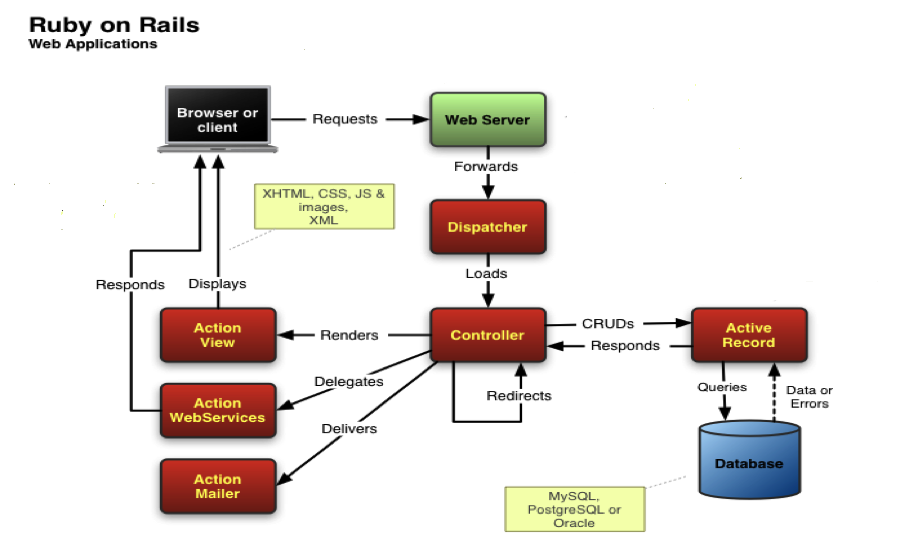
\includegraphics[width=0.5\linewidth]{rails_arch}
	\caption{Synoptique d'une application web en Ruby On Rails}
	\label{fig:railsarch}
\end{figure}

Le contrôleur s’occupe de l’accès aux données.  Nous implémentons aussi dans 
cette couche les algorithmes métier de notre système. Elle ne change pas si on modifie
l’interface utilisateur ou la façon d’accéder aux données nécessaire au fonctionnement 
de l’application.\\

L’interface utilisateur est l’interface web qui permet à l’utilisateur de piloter 
l’application et d’en recevoir des informations.
\section{Arborescence de l'application}

Nous  avons  dans  ce  chapitre  dévoilé   ce  qui  a  été  utilisé  pour  résoudre  la 
problématique  générale  du suivi des projets du courrier et d'archivage. Mais aussi, pour la satisfaction de chaque besoin émis par le cahier de charges.
Il ne nous reste plus qu’à présenter le résultat de tout cela dans le chapitre qui suit.

	\bigskip
\chapter{RÉSULTATS ET COMMENTAIRES}
	\bigskip
	
	\chapter*{Conclusion et Perceptives}\addcontentsline{toc}{chapter}{Conclusion}
	
	
\end{document}